\section{Třetí týden}

\subsection{Metoda nejmenších čtverců}

\begin{multicols}{2}
    \begin{tikzpicture}
        \draw[->] (-2,0) -- (2,0) node[right] {\(x\)};
        \draw[->] (0,-2) -- (0,2) node[above] {\(y\)};
        
        \draw[blue, thick] (-1.5,-1.5) -- (1.5,1.5) node[right] {\(L = \bc{Ax \mid x \in \R^n}\)};
    
        \filldraw[red, thick] (-1, 2) circle (2pt) node[above] {$b$};
        \filldraw[red, thick] (0.5, 0.5) circle (2pt) node[right] {$P_L (b)$};
        \draw[red, dashed] (-1, 2) -- (0.5, 0.5);
    \end{tikzpicture}

\columnbreak
    Pokud $b \in L$, řešíme úlohu $Ax = b$. \\Pokud $b \not\in L$, řešíme $Ax = P_L (b)$.
    \[
        \argmin_{x \in \R^n} \| Ax - b\| = \argmin_{x \in \R^n} \| Ax - b\|^2
    \]
\end{multicols}
Důkaz.

Chceme ukázat, že $\hat x \in \underset{x \in \R^n}{\argmin} \| Ax - b^2\| \iff A^T A \hat x = A^T b$.

\enquote{$\Rightarrow$}: Ať $A \hat x = P_L (b) \stackrel{\hyperref[varNer]{(2)}}{=} b - P_{L^\perp} (b) \quad / \cdot A^T$
\[
    A^T A \hat x = A^T  b - \underbrace{A^T P_{L^\perp} (b)}_{\stackrel{?}{=0}}
\]
\[
    \rightarrow \| A^T P_{L^\perp} (b)\|^2 = \langle A^T P_{L^\perp} (b), A^T P_{L^\perp} (b)\rangle = 
    \langle \underbrace{P_{L^\perp} (b)}_{\in L^\perp}, \underbrace{(A^T)^T (A^T P_{L^\perp} (b))}_{\in L}\rangle = 0. \qed
\]

\enquote{$\Leftarrow$}: Ať $A^T A \hat x = A^T b$.\\
Ať $x \in \R^n$.
\[
    0 = \langle \underbrace{x, A^T A \hat x - A^T b}_{A^T (A \hat x - b)}\rangle = 
    \langle \underbrace{(A^T)^T x}_L, A \hat x - b\rangle \implies A \hat x - b \in L^\perp
\]
\[
    \rightarrow b = \underbrace{A \hat x}_{\in L} + \underbrace{(b-A \hat x)}_{L^\perp} 
    \stackrel{\hyperref[ortoRoz]{(c)}}{\implies} A \hat x = P_L (b). \qed
\]

\subsection{Příklad výpočtu metody nejmenších čtverců}
$
A=
\begin{bmatrix}
    1 & 0 \\
    0 & 1 \\
    1 & 1
\end{bmatrix},
b=
\begin{bmatrix}
    1 \\
    1 \\
    1 
\end{bmatrix}$.

$A^T A \hat x = A^T b$

$A^T A = 
\begin{bmatrix}
    1 & 0 & 1 \\
    0 & 1 & 1
\end{bmatrix}
\begin{bmatrix}
    1 & 0 \\
    0 & 1 \\
    1 & 1
\end{bmatrix}
=
\begin{bmatrix}
    2 & 1 \\
    1 & 2 
\end{bmatrix} 
\rightarrow \det = 3 \implies \text{existuje inverze.}$
\\

$(A^T A)^{-1} = \frac{1}{3}
\begin{bmatrix}
    2 & -1 \\
    -1 & 2 
\end{bmatrix} \implies \hat x = (A^T A)^{-1}A^T b = \frac{1}{3}
\begin{bmatrix}
    2 & -1 \\
    -1 & 2 
\end{bmatrix}
\begin{bmatrix}
    1 & 0 & 1 \\
    0 & 1 & 1
\end{bmatrix}
\begin{bmatrix}
    1 \\
    1 \\
    1 
\end{bmatrix}\\ 
= \frac{1}{3}
\begin{bmatrix}
    2 & -1 \\
    -1 & 2 
\end{bmatrix}
\begin{bmatrix}
    2 \\
    2 
\end{bmatrix} = \frac{1}{3}
\begin{bmatrix}
    2 \\
    2 
\end{bmatrix}$.

\subsection{Příklad výpočtu metody nejmenších čtverců}
V rovině jsou dány body $(0, -\frac{1}{2})^T, (1, \frac{1}{3})^T$ a $(2, \frac{2}{3})^T$. Pomocí metody nejmenších 
čtverců proložme těmito body přímku o rovnici $y = kx + q$, kde $k ,q \in \R$.

\[
\begin{rcases*}
    0k + q = -\frac{1}{2} \\
    1k + q = \frac{1}{3} \\
    2k + q = \frac{2}{3}
\end{rcases*} 
A = 
\begin{bmatrix}
    0 & 1 \\
    1 & 1 \\
    2 & 1
\end{bmatrix},
b = 
\begingroup
    \renewcommand*{\arraystretch}{1.5}
    \begin{bmatrix}
        -\frac{1}{2} \\
        \phantom{-}\frac{1}{3} \\
        \phantom{-}\frac{2}{3}
    \end{bmatrix}
\endgroup
\]

$A^T A = 
\begin{bmatrix}
    0 & 1 & 2 \\
    1 & 1 & 1
\end{bmatrix}
\begin{bmatrix}
    0 & 1 \\
    1 & 1 \\
    2 & 1 
\end{bmatrix} =
\begin{bmatrix}
    5 & 3 \\
    3 & 3
\end{bmatrix}$

$(A^T A)^{-1} = \frac{1}{6}
\begin{bmatrix}
    \phantom{-}3 & -3 \\
    -3 & \phantom{-}5
\end{bmatrix}$

\[
    \hat x = \frac{1}{6}
    \begin{bmatrix}
        \phantom{-}3 & -3 \\
        -3 & \phantom{-}5
    \end{bmatrix}
    \begin{bmatrix}
        0 & 1 & 2 \\
        1 & 1 & 1
    \end{bmatrix}
    \begingroup
        \renewcommand*{\arraystretch}{1.5}
        \begin{bmatrix}
            -\frac{1}{2} \\
            \phantom{-}\frac{1}{3} \\
            \phantom{-}\frac{2}{3}
        \end{bmatrix}
    \endgroup = \frac{1}{6}
    \begin{bmatrix}
        \phantom{-}3 & -3 \\
        -3 & \phantom{-}5
    \end{bmatrix}
    \begingroup
        \renewcommand*{\arraystretch}{1.5}
        \begin{bmatrix}
            \frac{5}{3} \\
            \frac{1}{2}
        \end{bmatrix}
    \endgroup = \frac{1}{6}
    \begingroup
        \renewcommand*{\arraystretch}{1.5}
        \begin{bmatrix}
            \phantom{-}\frac{7}{2} \\
            -\frac{5}{2}
        \end{bmatrix}
    \endgroup = \frac{1}{12}
    \begin{bmatrix}
        \phantom{-}7 \\
        -5
    \end{bmatrix}.
\]

\subsection{Věta o oddělitelnosti bodu a konvexní množiny} \label{oddel}
\begin{multicols}{2}
    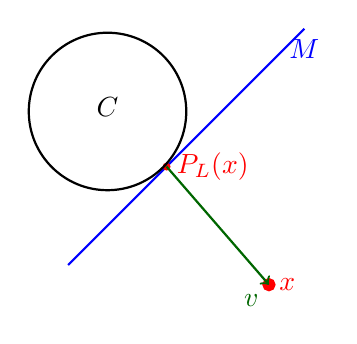
\begin{tikzpicture}  
        \draw[blue, thick] (-0.5,-0.5) -- (2.5,2.5) node[below]{$M$};

        \filldraw[red, thick] (2.05, -0.75) circle (2pt) node[right] {$x$};
        \filldraw[red, thick] (0.75, 0.75) circle (1pt) node[right] {$P_L (x)$};
        \draw[->][black!60!green, thick] (0.75, 0.75) -- (2.05, -0.75)node[below left]{$v$};
        \draw[black, thick] (0, 1.45) circle (1);
        \node at (0, 1.5) {$C$};
    \end{tikzpicture}

\columnbreak
    \hspace*{-2cm}
    $C \in \R^n$ je neprázdná uzavřená konvexní množina.
    \\
    \hspace*{-2cm}
    $x \in \R^n \setminus C \implies \text{existuje } v \in \R^n \setminus \bc{0}$ a $\alpha \in \R$ tak, že
    \\
    $\langle y, v\rangle \leq \alpha < \langle x, v\rangle, \quad \forall y \in C.$
\end{multicols}
Důkaz.\\
$v = x - P_L (x) \not=0$

\[
    \langle v, y\rangle = \langle v, P_L(x)\rangle \leq 0, \quad \forall y \in C.
\]
\[
    \langle y, v\rangle \leq \langle v, P_L (x)\rangle, \quad \forall y \in C.
\]
Položme $\alpha = \langle v, P_L (x)\rangle$.
\[
    \langle y, v\rangle \leq \alpha, \quad \forall y \in C.
\]
\[
    \langle x, v\rangle - \underbrace{\overbrace{\langle v, P_L (x)\rangle}^{\alpha}}_{\langle P_L(x), v\rangle} = 
    \langle \underbrace{x - P_L (x)}_{v}, v\rangle = \| v\|^2 > 0. \implies \alpha < \langle x, v\rangle. \qed
\]

\textbf{Důsledek:} Každá uzavřená konvexní množina v $\R^n$ je průnikem všech poloprostorů, které ji obsahují.

Důkaz sporem.

Ať neplatí: tj. existuje $C \in \R^n$ uzavřená konvexní množina tak, že není průnikem $P$ všech poloprostorů 
obsahujících $C$.

Pak $x \in P$ tak, že $x \not\in C$. Z věty o oddělitelnosti bodu a konvexní množiny existuje poloprostor $M$ takový,
že $C \subseteq M$ a $x \not= M$. Ale to je ve sporu s tím, že $x \in P. \qed$

\subsection{Příklad na použití věty o oddělitelnosti nadrovinou}
Nechť $A = 
\begin{bmatrix}
    1 & 1 \\
    2 & -1    
\end{bmatrix}$ a $b\in \R^2$. Označme
\begin{align*}
    C &= \bc{Ax \middle| x \in \R^2_+} = \bc{\alpha 
    \begin{bmatrix}
        1\\
        2    
    \end{bmatrix} + \beta
    \begin{bmatrix}
        \phantom{-}1\\
        -1
    \end{bmatrix} \mid \alpha, \beta \geq 0} \\
    K &= \bc{y \in \R^2 \mid A^T y \leq 0} \\
    &= \left\{y \in \R^2 \,\middle|\, \left\langle 
    \begin{bmatrix}
        1 \\
        2    
    \end{bmatrix}, y\right\rangle \leq 0,
    \left\langle 
    \begin{bmatrix}
        \phantom{-} 1 \\
        -1
    \end{bmatrix},y \right\rangle \leq 0\right\}.
\end{align*}

\begin{tikzpicture}[scale=2] % TODO: dodělat vektor b, který je mezi K a C
    \draw[->] (0,-2) -- (0,2) node[above] {\(y\)};
    \fill[green, opacity=0.3, pattern=north west lines] (0,0) -- (1,2) -- (1,-2) -- cycle;
    \fill[green, opacity=0.3, pattern=north west lines] (1,0) rectangle (2,2);
    \fill[green, opacity=0.3, pattern=north west lines] (1,0) rectangle (2,-2);

    \draw[black!40!yellow, semithick] (-0.5/4, 0.25/4) -- (-0.25/4, 0.75/4);
    \draw[black!40!yellow, semithick] (0.25/4, 0.5/4) -- (-0.25/4-0.005, 0.75/4);

    \draw[black!40!yellow, semithick] (-0.5/4, -0.25/4) -- (-0.25/4, -0.75/4);
    \draw[black!40!yellow, semithick] (0.25/4, -0.5/4) -- (-0.25/4-0.005, -0.75/4);

    \draw[black!30!blue, thick] (-2,-1) -- (0,0) node[above] {};
    \draw[black!30!blue, thick] (-2,1) -- (0,0) node[below] {};
    \fill[blue, opacity=0.3, pattern=north east lines] (0,0) -- (-2,1) -- (-2,-1) -- cycle;
    
    \draw[->][black!40!green, thick] (0,0) -- (1,2) node[above] {};
    \draw[->][black!40!green, thick] (0,0) -- (1,-2) node[below] {};

    \draw[black!40!green, thick] (1.2,1.8) node{$C$}; 
    \draw[black!30!blue, thick] (-1.8,0.7) node{$K$}; 

    \draw[->] (-2,0) -- (2,0) node[right] {\(x\)};
    
\end{tikzpicture}

Vždy nastane jeden z případů:
\begin{enumerate}[(a)]
    \item $b \in C$
    \item $b \not\in C$ - existuje nenulový vektor $y \in K$ svírající s $b$ úhel $\varphi \in [0, \frac{\pi}{2})$.
\end{enumerate}

\subsection{Lemma neprázdné uzavřené konvexní}
Jestliže $A \in \mathbb{M}_{m,n}(\R)$, pak $\bc{Ax \mid x \in \R_+^n}$ je neprázdná uzavřená konvexní množina.

Důkaz.
\begin{itemize}
    \item neprázdná - vždy obsahuje alespoň $0$,
    \item konvexní - lineární zobrazení (matice) zachovává konvexitu,
    \item uzavřenost dokazovat nebudeme.
\end{itemize}

\subsection{Farkasovo lemma}
Výslovnost [farkášovo].

Je-li $A \in \mathbb{M}_{m,n}(\R)$ a $b \in \R^m$, pak platí právě jedno z následujících tvrzení:
\begin{enumerate}[(a)]
    \item Existuje $x \in \R^n$ tak, že $Ax = b$ a $x \geq 0$.
    \item Existuje $y \in \R^m$ tak, že $A^Ty \leq 0$ a $\langle y, b\rangle > 0$.
\end{enumerate}

Důkaz.

\enquote{$(a) \implies \lnot (b)$}:\\
Ať $x \in \R^n_+$ a $y \in \R^m$ tak, že $Ax = b$ a $A^T y \leq 0$.
\[
    \langle y, b\rangle \stackrel{b= Ax}{=} \langle y, Ax\rangle = \langle \underbrace{A^Ty}_{\leq 0}, \underbrace{x}_{\geq 0}\rangle \leq 0. \qed 
\]

\enquote{$\lnot (a) \implies (b)$}:\\
Ať $C = \bc{Ax \mid x \in \R^n_+} \implies b \not\in C$, $C \dots$ uzavřená neprázdná konvexní množina.

$\stackrel{\text{\hyperref[oddel]{oddělitelnost}}}{\implies}$ existuje $y \in \R^m \setminus \bc{0}, \alpha \in \R$ tak, 
že: $\langle Ax, y\rangle \leq \alpha < \langle b, y\rangle, \quad \forall x \in \R^n_+$.

Začněme s $\alpha < \langle b, y\rangle$. Chceme, aby $\langle b, y\rangle$ byl kladný. Pak nám $y$ bude svírat ostrý 
úhel s $b$. 

Protože v $0 \in C$, je $0 \leq \alpha < \langle b,y \rangle$ (za $Ax$ dosadíme $0$, takže budeme mít $\langle 0, y\rangle$).

Teď musíme dokázat, že $y$ skutečně řeší zadanou soustavu nerovnic.

Víme tedy, že:
\begin{align*}
    \langle Ax, y\rangle \leq \alpha,  &\quad \forall x \in \R^n_+ \\
    \langle x, A^T y\rangle \leq \alpha, &\quad \forall x \in \R^n_+
\end{align*}
Odtuď $\langle x, A^T y\rangle \leq 0, \quad \forall x \in \R^n_+$, neboť:

Ať $\tilde x \in \R^n_+$ je takový, že $\langle \tilde x, A^T y\rangle > 0$.\\
Pak $\langle \underbrace{\lambda \tilde x}_{\lambda > 0, \text{ tedy } \lambda \tilde x \in \R^n_+}, A^T y\rangle = 
\lambda \underbrace{\langle \tilde x, A^T y\rangle}_{> 0} \rightarrow + \infty$, pro $\lambda \rightarrow + \infty$.
Což je spor s $\langle x, A^T y\rangle \leq \alpha, \forall x \in \R^n_+$.

Ať $e_1=
\begin{bmatrix}
    1 \\
    0 \\
    \vdots \\
    0
\end{bmatrix}, \dots, e_n = 
\begin{bmatrix}
    0 \\
    \vdots \\
    1
\end{bmatrix}$. Pak $(A^T y)_i \leq 0, \quad \forall i \in \bc{1, \dots, n}$, neboť $(A^T y)_i = \langle e_i, A^T y\rangle. \qed$

\subsection{Krajní body konvexní množiny}

\begin{multicols*}{2}
    \begin{tikzpicture}
        \coordinate (A) at (0,0);
        \coordinate (B) at (5,0);
        \coordinate (C) at (2.5,4);
    
        \draw[thick] (A) -- (B) -- (C) -- cycle;
    
        \coordinate (D) at (3, 2);
        \coordinate (E) at (2, 3);
    
        \draw[thick] (D) -- (E);
    
        \draw (2.9, 1.9) -- (3.1,2.1);
        \draw (1.9, 2.9) -- (2.1,3.1);
    
        \coordinate (M) at ($(D)!0.5!(E)$);
        \fill[black] (M) circle (2pt);
    
        \fill[black!40!green] (B) circle(2pt);
    \end{tikzpicture}

\columnbreak
    Mějme konvexní množinu. Když sestrojíme libovolnou nedegenerativní (tzn. netriviální = není to pouze bod) úsečku,
    vždy nalezneme bod, který bude ležet přesně uprostřed této úsečky.

    Co když ale vezmeme například \textcolor{black!40!green}{zelený bod} vyznačený na nákresu? V takovém případě nejsme
    schopni sestroji nedegenerativní úsečku, na jejímž středu by ležel tento bod.
\end{multicols*}
Definujme: Krajní bod $x \in C$ konvexní množiny $C \subseteq \R^n$ je takový bod, pro který neexistují dva 
\underline{různé} body $y, z$ tak, že
\[
    x = \frac{1}{2}y + \frac{1}{2}z \text{.}
\]

$\text{ext}(C) \dots$ množina všech krajních (extremálních) bodů

\subsection{Kreinova-Milmanova věta}
Jestliže $C \subseteq \R^n$ je kompaktní (tj. omezená a uzavřená) konvexní množina, pak $C = \text{conv}(\text{ext}(C))$.\\
Důkaz vynecháme.

Kompaktnost je důležitá.
\begin{itemize}
    \item Interval $(0,1)$ není uzavřený a ext$((0,1)) = \emptyset$.
    \item Množina $\R_+^2$ není omezená a ext$(\R_+^2) = \bc{0}$.
\end{itemize}

\subsection{Výpočet gradientu skalárního součinu}
Nalezněte $\nabla f(x)$ a $\nabla^2 f(x)$, jestliže
\begin{enumerate} [(a)]
    \item $f(x) = \langle x, c\rangle$, kde $c \in \R^n$;
    \item $f(x) = \langle Ax, x\rangle$, kde $A \in \M_n (\R)$. Určete také $\nabla f(x)$ a $\nabla^2 f(x)$ za dodatečného
    předpokladu, že $A$ je symetrická matice.
\end{enumerate}

(a) 
\[ 
    \frac{\partial f}{\partial x_k} = \frac{\partial}{\partial x_k} \sum_{i=1}^{n} x_i c_i \overset{\text{limita}}{=} 
    \sum_{i=1}^{n} c_i \frac{\partial x_i}{\partial x_k} = \sum_{i=1}^{n}c_i \delta_{ik} \overset{\text{rozvoj}}{=} c_k
\]
$\implies \nabla f(x) = 
\begin{bmatrix}
    c_1 \\
    \vdots \\
    c_k    
\end{bmatrix} = c$; $\implies \nabla^2 f(x) = 0$, kde $\delta_{ik} = 
\begin{cases}
    1, \text{ pokud } i = k, \\
    0, \text{ pokud } i \not= k.
\end{cases}$

(b)
\[ 
    \frac{\partial f}{\partial x_k} = \frac{\partial}{\partial x_k} \sum_{i=1}^{n} 
    \underbrace{\left[\sum_{j=1}^{n} a_{ij}x_j\right]}_{(Ax)_i}x_i = \sum_{i,j=1}^{n} a_{ij} 
    \underbrace{\left( \frac{\partial x_i}{\partial x_k}x_j + x_i \frac{\partial x_j}{\partial x_k}\right)}_{\text{derivace součinu}}
    = \sum_{i,j=1}^{n} a_{ij} (\delta_{ik} x_j + x_i \delta_{jk})
\]
\[
    = \sum_{i,j=1}^{n} a_{ij}\delta_{ik}x_j + a_{ij}\delta_{jk}x_i = \underbrace{\sum_{j=1}^{n}a_{kj} x_j}_{(Ax)_k} + 
    \underbrace{\sum_{i=1}^{n}a_{ik}x_i}_{(A^Tx)_k}
\]
$\implies \nabla f(x) = Ax + A^Tx$ (Speciálně: $\nabla f(x) = 2Ax$ pro $A = A^T$)\\
\[
    \frac{\partial^2 f}{\partial x_k x_l} = \sum_{j=1}^{n} a_{kj} \delta_{jl} + \sum_{i=1}^{n}a_{ik} \delta_{il} = 
    a_{kl} + a_{lk}
\]
$\implies \nabla^2 f(x) = A + A^T$

\newpage
\subsection{Ověření konvexnosti množiny}
\begin{multicols}{2}
    Je množina $M = \bc{
    \begin{bmatrix}
        x \\
        y
    \end{bmatrix} \in \R^2 \mid |x| + |y| \leq 1} \text{konvexní?}$

\columnbreak

\hspace*{2cm}
    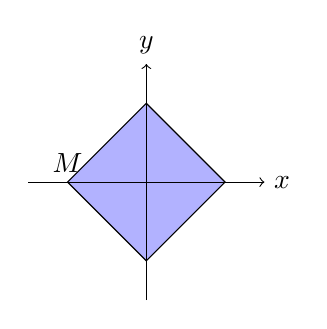
\begin{tikzpicture}
        \filldraw[fill=blue!30, draw=black] (-1,0) -- (0,-1) -- (1,0) -- (0,1) -- cycle node[above]{$M$};
        \draw[->] (-1.5,0) -- (1.5,0) node[right] {$x$};
        \draw[->] (0,-1.5) -- (0,1.5) node[above] {$y$};
    \end{tikzpicture}
\end{multicols}

1. způsob - dle definice
\[
    \lambda 
    \begin{bmatrix}
        x\\
        y     
    \end{bmatrix} + (1-\lambda)
    \begin{bmatrix}
        a\\
        b
    \end{bmatrix} = 
    \begin{bmatrix}
        \lambda x  + (1-\lambda) a \\
        \lambda y + (1-\lambda) b
    \end{bmatrix} \overset{?}{\in} M, \lambda \in [0,1].
\]
\[
    |\lambda x + (1-\lambda)a| + |\lambda y + (1-\lambda)b| \leq 
    \underbrace{\lambda |x| + (1-\lambda)|a| + \lambda |y| + (1-\lambda)|b|}_{\lambda
    \underbrace{(|x|+|y|)}_{\leq1} + (1-\lambda)\underbrace{(|a|+|b|)}_{\leq 1}} \leq \lambda + 1 - \lambda = 1 \qed
\]
$M$ je konvexní.

2. způsob - úvaha nad vlastnostmi

$|x|$ je konvexní, $|y|$ je konvexní. Součet zachovává konvexitu, tedy i $|x| + |y|$ je konvexní.

\subsection{Práce s maticemi}
Je dána matice $A \in \M_{m,n} (\R)$. Ať $L = \bc{Ax \mid x \in \R^n}$. 

Ukažte, že $A$ má lineárně nezávislé sloupce $\iff$ $A^T A$ je invertibilní.

Pomocný důkaz.\\
Ukažme, že: $\ker(A) = \ker(A^T A)$\\
Chci: $\ker(A) \subseteq \ker(A^TA)$
\begin{flalign*}
    x \in \ker(A) \Rightarrow  Ax &= 0 \quad / \cdot A^T& \\
    A^TA &= 0 \Rightarrow x \in \ker(A^TA) \qed
\end{flalign*}
Chci: $\ker(A^TA) \subseteq \ker(A)$
\begin{flalign*}
    x \in \ker(A^TA) \Rightarrow  A^TAx = 0 \Rightarrow 0 &= \langle A^T A x, x\rangle& \\
    &= \langle Ax , Ax\rangle &\\
    &= \| Ax\|^2 \Rightarrow Ax = 0 \Rightarrow x \in \ker(A) \qed
\end{flalign*}
Konec pomocného důkazu.

$A$ má lineárně nezávislé sloupce $\iff \bc{0} = \ker(A) = \ker(A^TA) \iff A^TA$ je invertibilní (protože $A^TA$ je 
čtvercová a $A^TA$ je prosté).

\newpage
\subsection{Proložení bodů pomocí MNČ}
Jsou dány body $a = 
\begin{bmatrix}
    -2 \\
    -1
\end{bmatrix}, b=
\begin{bmatrix}
    -1 \\
    -2
\end{bmatrix}, c=
\begin{bmatrix}
    0 \\
    0
\end{bmatrix}, d=
\begin{bmatrix}
    1 \\
    2
\end{bmatrix}$. Metodou nejmenších čtverců proložte těmito body graf
\begin{enumerate}[(a)]
    \item afinní funkce $f(x) = \alpha x + \beta$, kde $\alpha, \beta \in \R$;
    \item funkce $f(x) = \alpha x^2 + \beta x + \gamma$, kde $\alpha, \beta, \gamma \in \R$.
\end{enumerate}
(a) 
\begin{flalign*}
    &\begin{aligned}
        -2\alpha + \beta &= -1 \\
        - \alpha + \beta &= -2 \\
        0 \alpha + \beta &= 0 \\
          \alpha + \beta &= 2
    \end{aligned}
    \iff 
    \begin{aligned}
        A 
        \begin{bmatrix}
            \alpha \\
            \beta    
        \end{bmatrix} = b, \text{ kde } A = 
        \begin{bmatrix}
            -2 & 1 \\
            -1 & 1 \\
            \phantom{-}0 & 1 \\
            \phantom{-}1 & 1
        \end{bmatrix}\text{, } b=
        \begin{bmatrix}
            -1 \\
            -2 \\
            \phantom{-}0 \\
            \phantom{-}2
        \end{bmatrix}.
    \end{aligned}
\end{flalign*}
$A^T A 
\begin{bmatrix}
    \alpha \\
    \beta
\end{bmatrix} = A^T b$. $A$ má lineárně nezávislé sloupce $\Rightarrow$ $(A^T A)^{-1}$ existuje.\\
Pak: $
\begin{bmatrix}
    \alpha \\
    \beta    
\end{bmatrix} = (A^TA)^{-1} A^Tb$.

$A^T A = 
\begin{bmatrix}
    -2 & -1 & 0 & 1 \\
    \phantom{-}1 & \phantom{-}1 & 1 & 1
\end{bmatrix}
\begin{bmatrix}
    -2 & 1 \\
    -1 & 1 \\
    \phantom{-}0 & 1 \\
    \phantom{-}1 & 1 
\end{bmatrix} = 
\begin{bmatrix}
    \phantom{-}6 & -2 \\
    -2 & \phantom{-}4
\end{bmatrix} \Rightarrow (A^T A)^{-1} = \frac{1}{20}
\begin{bmatrix}
    4 & 2 \\
    2 & 6
\end{bmatrix}$.

$\begin{bmatrix}
    \alpha \\
    \beta
\end{bmatrix} = \frac{1}{10}
\begin{bmatrix}
    2 & 1 \\
    1 & 3
\end{bmatrix}
\begin{bmatrix}
    -2 & -1 & 0 & 1 \\
    \phantom{-}1 & \phantom{-}1 & 1 & 1
\end{bmatrix}
\begin{bmatrix}
    -1 \\
    -2 \\
    \phantom{-}0 \\
    \phantom{-}2
\end{bmatrix} = \frac{1}{10}
\begin{bmatrix}
    2 & 1 \\
    1 & 3
\end{bmatrix}
\begin{bmatrix}
    \phantom{-}6 \\
    -1
\end{bmatrix} = \frac{1}{10}
\begin{bmatrix}
    11 \\
    3
\end{bmatrix}$
$\Rightarrow \alpha = \frac{11}{10}$; $\beta = \frac{3}{10}$.

(b)
\begin{flalign*}
    &\begin{aligned}
        4\alpha           - 2\beta           + \gamma &= -1 \\
        \phantom{0}\alpha - \phantom{0}\beta + \gamma &= -2 \\
        0\alpha           + 0\beta           + \gamma &= 0 \\
        \phantom{0}\alpha + \phantom{0}\beta + \gamma &= 2
    \end{aligned}
    \iff 
    \begin{aligned}
        A 
        \begin{bmatrix}
            \alpha \\
            \beta    
        \end{bmatrix} = b, \text{ kde } A = 
        \begin{bmatrix}
            4 & -2 & 1 \\
            1 & -1 & 1\\
            0 & \phantom{-}0 & 1\\
            1 & \phantom{-}1 & 1
        \end{bmatrix}\text{, } b=
        \begin{bmatrix}
            -1 \\
            -2 \\
            \phantom{-}0 \\
            \phantom{-}2
        \end{bmatrix}.
    \end{aligned}
\end{flalign*}
$A$ má lineárně nezávislé sloupce $\Rightarrow$ $A^TA$ je invertibilní.

$A^T A = 
\begin{bmatrix}
    \phantom{-}4 & \phantom{-}1 & 0 & 1\\
    -2           & -1           & 0 & 1 \\
    \phantom{-}1 & \phantom{-}1 & 1 & 1
\end{bmatrix}
\begin{bmatrix}
    4 & -2 & 1 \\
    1 & -1 & 1\\
    0 & \phantom{-}0 & 1\\
    1 & \phantom{-}1 & 1
\end{bmatrix} = 
\begin{bmatrix}
    \phantom{-}18 & -8           & \phantom{-}6 \\
    -8            & \phantom{-}6 & -2 \\
    \phantom{-}6  & -2           & \phantom{-}4
\end{bmatrix} \Rightarrow (A^T A)^{-1} = \frac{1}{20}
\begin{bmatrix}
    \phantom{-}5 &  \phantom{-}5 & -5\\
    \phantom{-}5 &  \phantom{-}9 & -3\\
    -5           & -3            &  \phantom{-}11
\end{bmatrix}$.

$\begin{bmatrix}
    \alpha \\
    \beta \\
    \gamma
\end{bmatrix} = \frac{1}{20}
\begin{bmatrix}
    \phantom{-}5 &  \phantom{-}5 & -5\\
    \phantom{-}5 &  \phantom{-}9 & -3\\
    -5           & -3            &  \phantom{-}11
\end{bmatrix}
\begin{bmatrix}
    4 \\
    2 \\
    1
\end{bmatrix} = \frac{1}{20} 
\begin{bmatrix}
    \phantom{-}25\\
    \phantom{-}35\\
    -15
\end{bmatrix} = \frac{1}{4}
\begin{bmatrix}
    \phantom{-}5\\
    \phantom{-}7\\
    -3
\end{bmatrix}$ $\Rightarrow \alpha = \frac{5}{4}$; $\beta = \frac{7}{4}$; $\gamma = \frac{-3}{4}$.

\newpage
\subsection{Formulace úlohy MNČ}
Ať závislost výstupního signálu $(y_n)_{n=0}^\infty$ systému na vstupním signálu $(x_n)_{n=0}^\infty$ je dána konvolucí
posloupnosti $(x_n)_{n=0}^\infty$ s posloupností $(h_n)_{n=0}^\infty$ ($(h_n)_{n=0}^\infty$ popisuje odezvu systému
na jednotkový impuls), tj.  $y_n = \sum_{i=0}^{n}h_i x_{n-i}$. Předpokládejte dále, že $h_n = 0$ pro všechna $n \geq 4$.
Měřením byla zjištěna hodnota koeficientů $y_0, \dots, y_{20}$ výstupního signálu, když na vstupu byl signál s počátečními
koeficienty $x_0, \dots, x_{20}$. Formulujte úlohu nejmenších čtverců pro nalezení koeficientů $h_0, h_1, h_2, h_3$.

\begin{multicols}{2}
    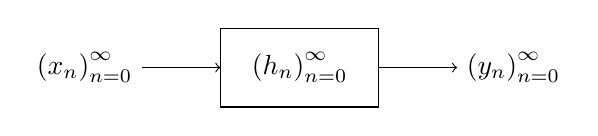
\begin{tikzpicture}
        \node[draw, rectangle, minimum width=2cm, minimum height=1cm] (box) 
            {\(\left( h_n \right)_{n=0}^{\infty}\)};
    
        \draw[->] (-2,0) node[left] {\(\left( x_n \right)_{n=0}^{\infty}\)}
            -- (box.west);
    
        \draw[->] (box.east) -- (2,0) node[right] {\(\left( y_n \right)_{n=0}^{\infty}\)};
    \end{tikzpicture}

    $y_k = \sum_{l=0}^k h_l x_{k-l} = h_0 x_k + \dots + h_k x_0$

    předpokládejme: $h_l = 0 \, \forall l \geq 4$. 
\columnbreak

    \begin{align*}
        y_0 &= h_0 x_0 \\
        y_1 &= h_1 x_0 + h_0 x_1 \\
        y_2 &= h_2 x_0 + h_1 x_1 + h_0 x_2 \\
        y_3 &= h_3 x_0 + h_2 x_1 + h_1 x_2 + h_0 x_3 \\
        y_4 &= h_3 x_1 + h_2 x_2 + h_3 x_3 + h_0 x_4 \\
        & \vdots \\
        y_{20} &= h_3 x_{17} + h_2 x_{18} + h_1 x_{19} + h_0 x_{20}
    \end{align*}
\end{multicols}
Minimalisujme $f(x) = \| Ax + b\|^2$, kde
\[
    A = 
    \begin{bmatrix}
        x_0 & 0 & 0 & 0 \\
        x_1 & x_0 & 0 & 0 \\
        x_2 & x_1 & x_0 & 0 \\
        x_3 & x_2 & x_1 & x_0 \\
        \vdots & \vdots & \vdots & \vdots \\
        x_{20} & x_{19} & x_{18} & x_{17}
    \end{bmatrix}\text{; } b = 
    \begin{bmatrix}
        y_0 \\
        y_1 \\
        \vdots \\
        y_{20}
    \end{bmatrix}.
\]
